\section{posix\-Account Class Reference}
\label{classposixAccount}\index{posixAccount@{posixAccount}}
posix\-Account plugin  


Inheritance diagram for posix\-Account::\begin{figure}[H]
\begin{center}
\leavevmode
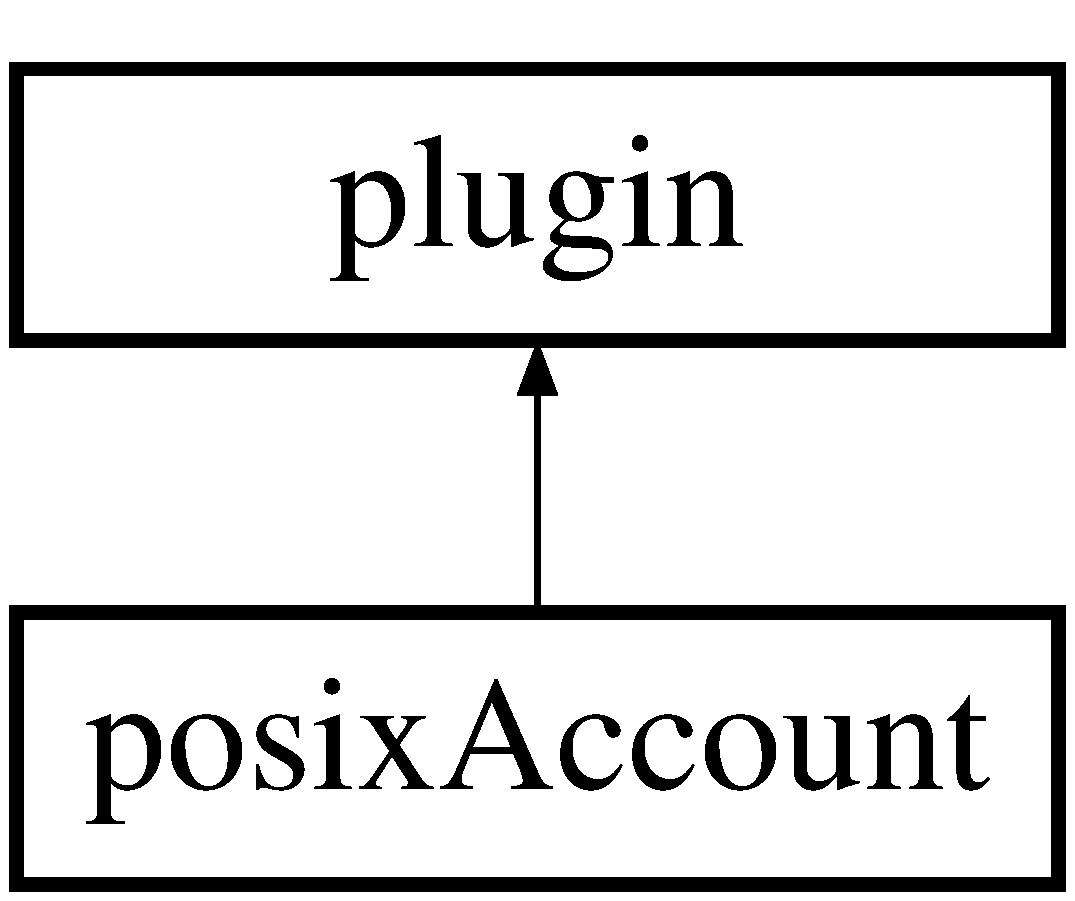
\includegraphics[height=2cm]{classposixAccount}
\end{center}
\end{figure}
\subsection*{Public Member Functions}
\begin{CompactItemize}
\item 
{\bf posix\-Account} (\${\bf dn}=NULL)\label{classposixAccount_a0}

\item 
{\bf execute} ()
\begin{CompactList}\small\item\em execute plugin \item\end{CompactList}\item 
{\bf remove\_\-from\_\-parent} ()\label{classposixAccount_a2}

\item 
{\bf save\_\-object} ()\label{classposixAccount_a3}

\item 
{\bf save} ()\label{classposixAccount_a4}

\item 
{\bf check} ()\label{classposixAccount_a5}

\item 
{\bf add\-Group} (\$groups)\label{classposixAccount_a6}

\item 
{\bf del\-Group} (\$groups)\label{classposixAccount_a7}

\item 
{\bf adapt\_\-from\_\-template} (\${\bf dn})\label{classposixAccount_a8}

\end{CompactItemize}
\subsection*{Public Attributes}
\begin{CompactItemize}
\item 
{\bf home\-Directory} = \char`\"{}\char`\"{}\label{classposixAccount_o0}

\item 
{\bf login\-Shell} = \char`\"{}/bin/bash\char`\"{}\label{classposixAccount_o1}

\item 
{\bf uid\-Number} = \char`\"{}\char`\"{}\label{classposixAccount_o2}

\item 
{\bf gid\-Number} = \char`\"{}\char`\"{}\label{classposixAccount_o3}

\item 
{\bf gecos} = \char`\"{}\char`\"{}\label{classposixAccount_o4}

\item 
{\bf shadow\-Min} = \char`\"{}0\char`\"{}\label{classposixAccount_o5}

\item 
{\bf shadow\-Max} = \char`\"{}0\char`\"{}\label{classposixAccount_o6}

\item 
{\bf shadow\-Warning} = \char`\"{}0\char`\"{}\label{classposixAccount_o7}

\item 
{\bf shadow\-Last\-Change} = \char`\"{}0\char`\"{}\label{classposixAccount_o8}

\item 
{\bf shadow\-Inactive} = \char`\"{}0\char`\"{}\label{classposixAccount_o9}

\item 
{\bf shadow\-Expire} = \char`\"{}0\char`\"{}\label{classposixAccount_o10}

\item 
{\bf gosa\-Default\-Printer} = \char`\"{}\char`\"{}\label{classposixAccount_o11}

\item 
{\bf gosa\-Default\-Language} = \char`\"{}\char`\"{}\label{classposixAccount_o12}

\item 
{\bf gosa\-Host\-ACL} = array()\label{classposixAccount_o13}

\item 
{\bf status} = \char`\"{}\char`\"{}\label{classposixAccount_o14}

\item 
{\bf login\-Shell\-List} = array()\label{classposixAccount_o15}

\item 
{\bf group\-Membership} = array()\label{classposixAccount_o16}

\item 
{\bf saved\-Group\-Membership} = array()\label{classposixAccount_o17}

\item 
{\bf saved\-Uid\-Number} = \char`\"{}\char`\"{}\label{classposixAccount_o18}

\item 
{\bf saved\-Gid\-Number} = \char`\"{}\char`\"{}\label{classposixAccount_o19}

\item 
{\bf use\_\-shadow\-Min} = \char`\"{}0\char`\"{}\label{classposixAccount_o20}

\item 
{\bf use\_\-shadow\-Max} = \char`\"{}0\char`\"{}\label{classposixAccount_o21}

\item 
{\bf use\_\-shadow\-Warning} = \char`\"{}0\char`\"{}\label{classposixAccount_o22}

\item 
{\bf use\_\-shadow\-Inactive} = \char`\"{}0\char`\"{}\label{classposixAccount_o23}

\item 
{\bf use\_\-shadow\-Expire} = \char`\"{}0\char`\"{}\label{classposixAccount_o24}

\item 
{\bf must\_\-change\_\-password} = \char`\"{}0\char`\"{}\label{classposixAccount_o25}

\item 
{\bf force\_\-ids} = 0\label{classposixAccount_o26}

\item 
{\bf printer\-List} = array()\label{classposixAccount_o27}

\item 
{\bf group\_\-dialog} = FALSE\label{classposixAccount_o28}

\item 
{\bf hosts\_\-dialog} = FALSE\label{classposixAccount_o29}

\item 
{\bf attributes}
\item 
{\bf objectclasses} = array(\char`\"{}posix\-Account\char`\"{}, \char`\"{}shadow\-Account\char`\"{})\label{classposixAccount_o31}

\end{CompactItemize}


\subsection{Detailed Description}
posix\-Account plugin 

\begin{Desc}
\item[Author:]Cajus Pollmeier $<${\tt pollmeier@gonicus.de}$>$ \end{Desc}
\begin{Desc}
\item[Version:]2.00 \end{Desc}
\begin{Desc}
\item[Date:]24.07.2003\end{Desc}
This class provides the functionality to read and write all attributes relevant for posix\-Accounts and shadow\-Accounts from/to the LDAP. It does syntax checking and displays the formulars required. 



\subsection{Member Function Documentation}
\index{posixAccount@{posix\-Account}!execute@{execute}}
\index{execute@{execute}!posixAccount@{posix\-Account}}
\subsubsection{\setlength{\rightskip}{0pt plus 5cm}posix\-Account::execute ()}\label{classposixAccount_a1}


execute plugin 

Generates the html output for this node 

Reimplemented from {\bf plugin} {\rm (p.\,\pageref{classplugin_a1})}.

\subsection{Member Data Documentation}
\index{posixAccount@{posix\-Account}!attributes@{attributes}}
\index{attributes@{attributes}!posixAccount@{posix\-Account}}
\subsubsection{\setlength{\rightskip}{0pt plus 5cm}posix\-Account::attributes}\label{classposixAccount_o30}


{\bf Initial value:}

\footnotesize\begin{verbatim} array("homeDirectory", "loginShell", "uidNumber", "gidNumber", "gecos",
                        "shadowMin", "shadowMax", "shadowWarning", "shadowInactive", "shadowLastChange",
                        "shadowExpire", "gosaDefaultPrinter", "gosaDefaultLanguage", "uid")
\end{verbatim}\normalsize 


Reimplemented from {\bf plugin} {\rm (p.\,\pageref{classplugin})}.

The documentation for this class was generated from the following file:\begin{CompactItemize}
\item 
class\_\-posix\-Account.inc\end{CompactItemize}
